\chapter{Neuronen, actiepotentialen en synapsen}\label{ch:b2:neurons-synapses}

Tik op de pees onder de knieschijf en het been schiet dertig milliseconden
later naar voren. In die tijd is in de dij een rekking waargenomen, heeft
een signaal een meter afgelegd naar het ruggenmerg, is het via één
verbinding naar een tweede cel overgestoken, heeft het een meter terug
afgelegd en een spier aan het samentrekken gezet --- de hele heen- en
terugweg sneller dan een knippering van het oog. Geen \omterm{def:b2:cell-signalling:kinds}{hormoon} zou dit
kunnen; het gebeurt door cellen die gebouwd zijn om te geleiden, en door een
signaal dat geen stof is die zich verplaatst, maar een golf van elektriciteit
die langs een membraan steeds opnieuw wordt opgewekt. Dit hoofdstuk gaat over
die cel en dat signaal: de spanning die een \omterm{def:b2:neurons-synapses:neuron}{neuron} over zijn membraan
handhaaft, de impuls die het afvuurt en hoe de impuls zich voortplant, en de
\omterm{def:b2:neurons-synapses:synapse}{synaps} waar het elektrische signaal in een chemisch signaal wordt omgezet en
weer terug.

\section{Het neuron}

\begin{definition}[Neuron, axon, zenuw]\label{def:b2:neurons-synapses:neuron}
\index{neuron}\index{axon}\index{dendriet}\index{myeline}\index{glia}
Een \emph{neuron} is een cel die gespecialiseerd is in signalering: een
cellichaam (\emph{soma}) met de kern, vertakte \emph{dendrieten} die
signalen ontvangen, en één enkel \emph{axon} --- een kabel van een tot twintig
micrometer dik en tot een meter lang --- dat zijn uitvoer naar
\emph{uiteinden} op andere cellen brengt. De menselijke hersenen tellen zo'n
$10^{11}$ neuronen, en elk daarvan vormt ongeveer duizend synapsen. Neuronen
zijn in de minderheid tegenover de \emph{glia}: astrocyten die ze voeden en
bufferen, microglia die over ze waken, en de cellen die axonen omwikkelen met
\emph{myeline} --- tientallen windingen van hun eigen membraan, vrijwel
zonder cytoplasma, die een isolerende schede vormen die ongeveer elke
millimeter onderbroken wordt bij de \emph{knopen van Ranvier}. Een
\emph{zenuw} is een bundel van duizenden axonen, sensorische en motorische,
die samen in bindweefsel lopen. Neuronen delen zich bij de volwassene niet
(op enkele uitzonderingen na), en een axon dat van zijn cellichaam wordt
afgesneden, sterft af; een neuron is een cel die een leven lang mee moet.
\end{definition}

\begin{omfigure}
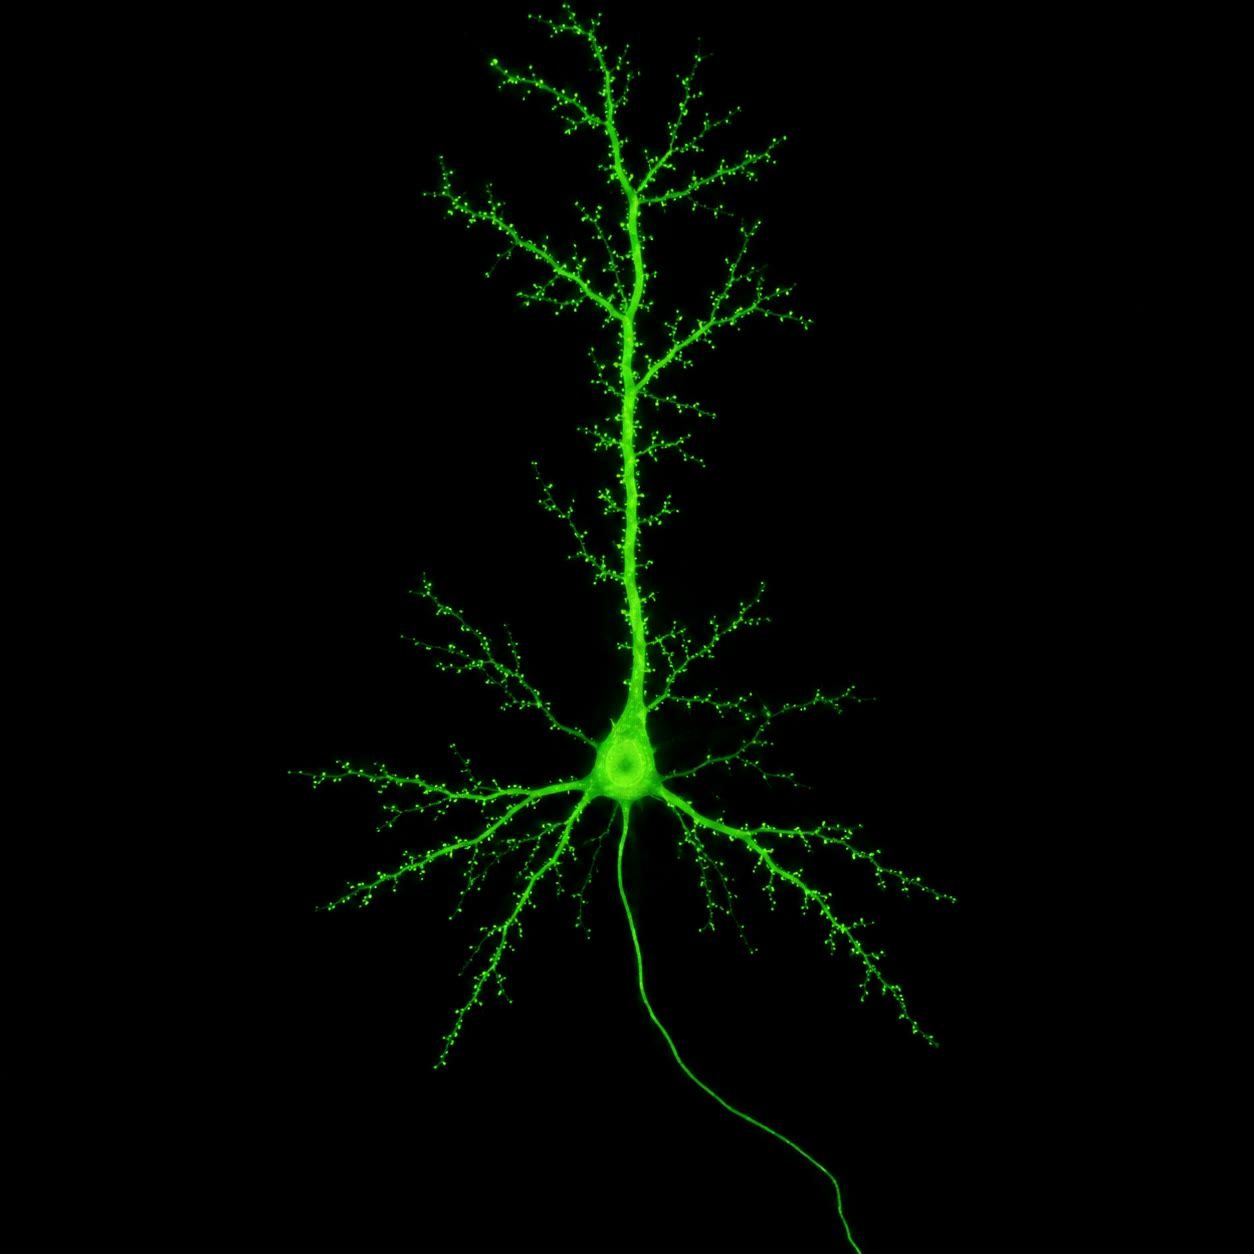
\includegraphics[width=0.4\linewidth]{images/book4/ai/b4-20-neuron-fluorescence.jpg}\hspace{0.05\linewidth}
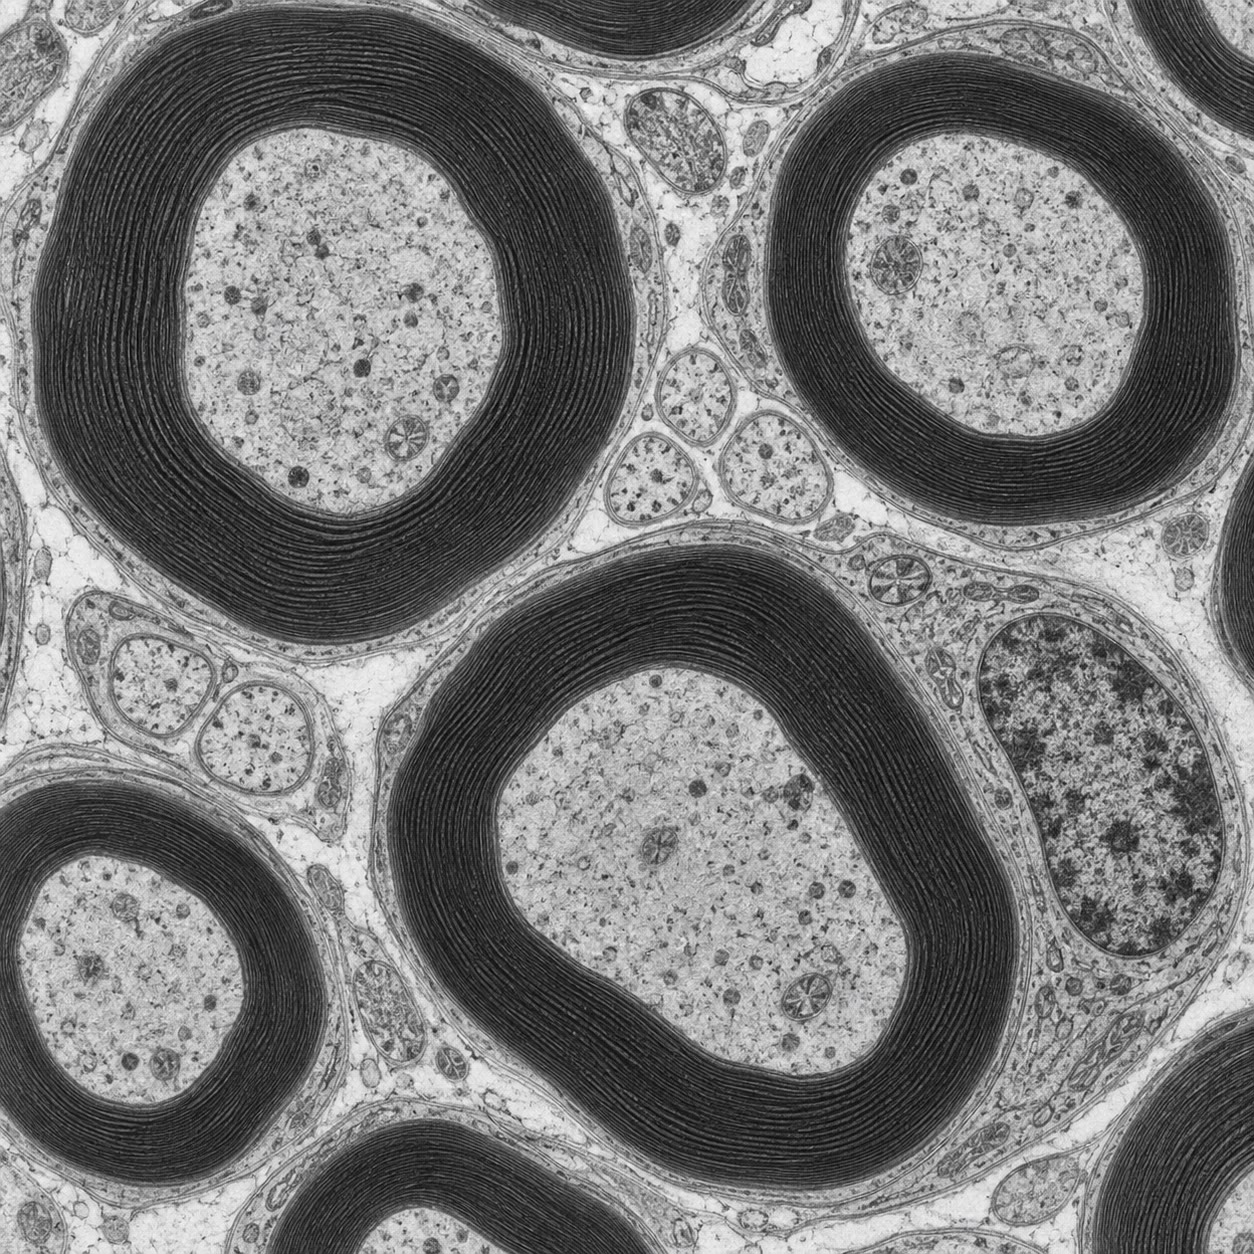
\includegraphics[width=0.4\linewidth]{images/book4/ai/b4-20-myelinated-axons-tem.jpg}

{\small Links: een piramidaal \omterm{def:b2:neurons-synapses:neuron}{neuron} gevuld met kleurstof --- het
cellichaam, de gedoornde \omterm{def:b2:neurons-synapses:neuron}{dendrieten} die ontvangen, en het dunne \omterm{def:b2:neurons-synapses:neuron}{axon} dat
aan de basis vertrekt. Rechts: \omterm{def:b2:neurons-synapses:neuron}{axonen} in dwarsdoorsnede onder de
elektronenmicroscoop, elk omwikkeld door de donkere spiraal van zijn myelineschede.}
\end{omfigure}

\section{De rustpotentiaal}

\begin{theorem}[De nernstpotentiaal]\label{thm:b2:neurons-synapses:nernst}
\index{nernstpotentiaal}\index{evenwichtspotentiaal}
Een membraan dat doorlaatbaar is voor één ion met lading $z$ en dat de
concentraties $c_{\text{uit}}$ en $c_{\text{in}}$ scheidt, komt tot rust op de
\emph{\omterm{thm:b2:neurons-synapses:nernst}{evenwichtspotentiaal}}, waarbij de elektrische kracht op het ion zijn
diffusie in evenwicht houdt:
\[
E = \frac{RT}{zF}\ln\frac{c_{\text{uit}}}{c_{\text{in}}} \approx \frac{\qty{61.5}{mV}}{z}\log_{10}\frac{c_{\text{uit}}}{c_{\text{in}}} \quad (\qty{37}{\celsius}).
\]
Een \omterm{def:b2:neurons-synapses:neuron}{neuron} houdt binnen \qty{140}{mmol/L} kalium tegenover
\qty{5}{mmol/L} buiten, en binnen \qty{15}{mmol/L} natrium tegenover
\qty{145}{mmol/L} buiten, gradiënten die door de natrium-kaliumpomp worden
opgebouwd ten koste van een derde van het ATP van de cel.
Dus $E_{\mathrm K} = 61.5\log_{10}(5/140) = \qty{-89}{mV}$ en
$E_{\mathrm{Na}} = 61.5\log_{10}(145/15) = \qty{+61}{mV}$: als het
membraan alleen kalium doorliet, zou het op \qty{-89}{mV} staan, als het
alleen natrium doorliet op \qty{+61}{mV}.
\end{theorem}
\begin{proof}
In evenwicht is de elektrochemische potentiaal van het ion aan beide
kanten gelijk: $RT\ln c_{\text{in}} + zFV_{\text{in}} = RT\ln
c_{\text{uit}} + zFV_{\text{uit}}$, dus $V_{\text{in}} -
V_{\text{uit}} = (RT/zF)\ln(c_{\text{uit}}/c_{\text{in}})$. Bij
\qty{310}{K} is $RT/F = \qty{26.7}{mV}$ en $\ln 10 \times 26.7 =
\qty{61.5}{mV}$. (Afgeleid in het deel van jaar 1 uit de
boltzmannverdeling; hier herhaald.)
\end{proof}

\begin{theorem}[De rustpotentiaal als gewogen gemiddelde]\label{thm:b2:neurons-synapses:chord}
\index{rustpotentiaal}\index{geleidbaarheid (membraan)}
Als het membraan meerdere ionen geleidt, elk met een geleidbaarheid $g_i$
(het gemak waarmee het doorgaat, bepaald door het aantal open kanalen),
is de stationaire potentiaal waarbij de stromen elkaar opheffen
\[
V = \frac{\sum_i g_i E_i}{\sum_i g_i},
\]
een gemiddelde van de evenwichtspotentialen, gewogen naar de
geleidbaarheden. In rust is het membraan van een \omterm{def:b2:neurons-synapses:neuron}{neuron} ongeveer twintig keer
doorlaatbaarder voor kalium dan voor natrium, dus $V \approx (20\times(-89) +
61)/21 = \qty{-82}{mV}$; met chloride en de kleine lekken meegeteld is de
\omterm{thm:b2:neurons-synapses:chord}{rustpotentiaal} \qty{-70}{mV}. Het membraan rust dicht bij $E_{\mathrm K}$
omdat de kaliumkanalen open staan; alles wat natriumkanalen opent, trekt het
naar $E_{\mathrm{Na}}$ --- en dat is het hele principe van de signalering
door zenuwen.
\end{theorem}
\begin{proof}
Elk ion voert een stroom $I_i = g_i(V - E_i)$ (de wet van Ohm, met de
drijvende kracht gemeten vanaf het eigen evenwicht van het ion). Bij een
stationaire potentiaal is de totale stroom nul: $\sum_i g_i(V - E_i) =
0$, waaruit $V\sum g_i = \sum g_iE_i$. (De volledige behandeling, waarin
de permeabiliteiten via de vergelijking van Goldman--Hodgkin--Katz
binnenkomen, geeft in eerste orde dezelfde weging.)
\end{proof}

\section{De actiepotentiaal}

\begin{proposition}[De impuls]\label{prop:b2:neurons-synapses:ap}
\index{actiepotentiaal}\index{spanningsafhankelijk kanaal}\index{drempel}\index{refractaire periode}
Het membraan van het \omterm{def:b2:neurons-synapses:neuron}{axon} bevat \emph{spanningsafhankelijke natriumkanalen},
die in rust gesloten zijn en door depolarisatie worden geopend. Als een
prikkel de potentiaal van \qty{-70}{mV} voorbij een \emph{drempel} rond
\qty{-55}{mV} brengt, gaan er genoeg open om meer natrium binnen te laten dan
het kaliumlek kan compenseren; de potentiaal stijgt, er gaan meer kanalen
open, en binnen een fractie van een milliseconde wordt het membraan naar
$E_{\mathrm{Na}}$ gedreven --- een \emph{positieve terugkoppeling} die
explosief is en alles-of-niets. De piek ligt rond \qty{+40}{mV} omdat de
natriumkanalen binnen een milliseconde na het openen \emph{inactiveren} en
omdat tragere \emph{spanningsafhankelijke kaliumkanalen} opengaan en de
potentiaal terugdrijven naar $E_{\mathrm K}$, voorbij de rustwaarde tot een
\emph{nahyperpolarisatie} voordat de kaliumkanalen sluiten. De
\emph{actiepotentiaal} duurt ongeveer een milliseconde; nog een milliseconde
of twee kunnen de geïnactiveerde natriumkanalen niet opnieuw opengaan (de
\emph{\omterm{prop:b2:neurons-synapses:ap}{refractaire periode}}), wat de vuurfrequentie beperkt tot enkele
honderden per seconde en de impuls dwingt in één richting te lopen.
Omdat hij alles-of-niets is, draagt de impuls geen informatie in zijn
grootte: het \omterm{def:b2:neurons-synapses:neuron}{neuron} codeert intensiteit in zijn \emph{frequentie}. Zo'n
$10^{4}$ natriumionen komen per impuls binnen en evenveel kaliumionen gaan
naar buiten --- een verwaarloosbare verandering van concentratie, die de
pomp op haar gemak herstelt.
\end{proposition}
\begin{proof}[Bewijsmateriaal]
Hodgkin en Huxley (1952) gebruikten het reuzenaxon van de pijlinktvis (een
halve millimeter dik, zodat er een draad in kon worden geschoven) en een
teruggekoppelde versterker die de membraanpotentiaal op elke gekozen waarde
vasthield (de \emph{spanningsklem}) terwijl de stroom werd geregistreerd die
daarvoor nodig was. Zo splitsten ze de stroom in een vroege inwaartse
component die verdween wanneer natrium uit het bad werd weggenomen, en een
latere uitwaartse component die door kalium werd gedragen; ze maten hoe elke
geleidbaarheid bij elke spanning in de tijd steeg en daalde; en door elk met
een paar vergelijkingen te beschrijven, berekenden ze de vorm, de drempel,
de snelheid en de \omterm{prop:b2:neurons-synapses:ap}{refractaire periode} van de actiepotentiaal uit alleen de
twee geleidbaarheden. Elke voorspelling klopte. De kanalen zelf werden
vijfentwintig jaar later gezien, één voor één, met de patch-clamptechniek;
tetrodotoxine (het gif van de kogelvis) blokkeert het natriumkanaal en heft
de impuls op, tetraethylammonium blokkeert het kaliumkanaal en verlengt de
impuls.
\end{proof}

\begin{omfigure}
\begin{tikzpicture}
\begin{axis}[
  width=0.9\linewidth, height=6.4cm,
  axis x line=bottom, axis y line=left,
  xmin=0, xmax=4, ymin=-100, ymax=60,
  xlabel={tijd (ms)}, ylabel={membraanpotentiaal (mV)},
  xlabel style={font=\small, at={(axis description cs:0.5,-0.1)}, anchor=north},
  ylabel style={font=\small},
  tick label style={font=\small}, xtick={0,1,2,3,4}, ytick={-90,-70,-55,0,40},
  legend style={font=\scriptsize, at={(0.97,0.95)}, anchor=north east, draw=none},
  clip=false,
]
\addplot[very thick, omDef] coordinates {(0,-70) (0.4,-70) (0.5,-64) (0.6,-55) (0.7,-30) (0.8,10) (0.9,35) (1.0,40) (1.1,30) (1.2,10) (1.35,-20) (1.5,-50) (1.7,-75) (1.9,-85) (2.2,-82) (2.6,-76) (3.2,-71) (4,-70)};
\addlegendentry{membraanpotentiaal}
\addplot[thick, omThm, dashed] coordinates {(0,0) (0.5,0) (0.6,5) (0.7,20) (0.8,35) (0.9,30) (1.0,20) (1.1,8) (1.2,3) (1.4,0) (4,0)};
\addlegendentry{$g_{\mathrm{Na}}$ (relatief)}
\addplot[thick, omProp, dashed] coordinates {(0,0) (0.6,0) (0.8,2) (1.0,8) (1.2,16) (1.4,20) (1.7,17) (2.0,10) (2.4,4) (3.0,1) (4,0)};
\addlegendentry{$g_{\mathrm K}$ (relatief)}
\draw[dashed, gray] (axis cs:0,-55) -- (axis cs:4,-55); \node[font=\scriptsize, anchor=south east] at (axis cs:4,-55) {drempel};
\draw[dashed, gray] (axis cs:0,-89) -- (axis cs:4,-89); \node[font=\scriptsize, anchor=south east] at (axis cs:3.7,-89) {$E_{\mathrm K}$};
\draw[<->, gray] (axis cs:1.0,50) -- (axis cs:2.5,50); \node[font=\scriptsize, anchor=south, gray] at (axis cs:1.75,50) {refractair};
\end{axis}
\end{tikzpicture}

{\small Een actiepotentiaal. Voorbij de drempel stijgt de
natriumgeleidbaarheid (rood) explosief en drijft de potentiaal naar
$E_{\mathrm{Na}}$; ze inactiveert terwijl de kaliumgeleidbaarheid
(oranje) stijgt en het membraan terugbrengt naar $E_{\mathrm K}$, met
een doorschieten voorbij de rustwaarde. Onder de drempellijn gebeurt er niets.}
\end{omfigure}

\section{Geleiding}

\begin{theorem}[De kabel en zijn lengteconstante]\label{thm:b2:neurons-synapses:cable}
\index{lengteconstante}\index{kabelvergelijking}\index{geleidingssnelheid}
Een \omterm{def:b2:neurons-synapses:neuron}{axon} is een lekkende kabel: stroom die op een punt wordt ingebracht,
loopt door het cytoplasma (weerstand $r_i$ per lengte-eenheid) en lekt weg
door het membraan (weerstand $r_m$ maal lengte-eenheid). Een constante
depolarisatie $V_0$ bij $x = 0$ neemt langs het \omterm{def:b2:neurons-synapses:neuron}{axon} af als
\[
V(x) = V_0\,e^{-x/\lambda}, \qquad \lambda = \sqrt{\frac{r_m}{r_i}} = \sqrt{\frac{R_m\,d}{4R_i}},
\]
waarin $d$ de diameter is en $R_m$, $R_i$ de soortelijke weerstanden van
het membraan en het cytoplasma. De \emph{\omterm{thm:b2:neurons-synapses:cable}{lengteconstante}}
$\lambda$ is de afstand waarover een passief signaal tot een derde daalt:
ongeveer \qty{0.5}{mm} voor een \omterm{def:b2:neurons-synapses:neuron}{axon} van \qty{1}{\micro m}, groeiend met
de wortel uit de diameter. Een actiepotentiaal plant zich voort doordat de
depolarisatie aan zijn front, die zich passief ongeveer $\lambda$ vooruit
verspreidt, het volgende stuk membraan tot de drempel brengt, dat hem op
volle grootte opnieuw opwekt; hoe verder vooruit hij reikt, hoe sneller de
golf, zodat ook de \omterm{thm:b2:neurons-synapses:cable}{geleidingssnelheid} ruwweg groeit als $\sqrt{d}$ --- van
\qty{1}{m/s} in een dunne ongemyeliniseerde vezel tot \qty{20}{m/s} in het
reuzenaxon van de pijlinktvis.
\end{theorem}
\begin{proof}
Zij $i(x)$ de axiale stroom en $V(x)$ de depolarisatie van het membraan. De
wet van Ohm langs het axoplasma geeft $\mathrm{d}V/
\mathrm{d}x = -r_i\,i$; ladingsbehoud, met het lek door het membraan,
geeft $\mathrm{d}i/\mathrm{d}x = -V/r_m$. Door combinatie volgt
$\mathrm{d}^{2}V/\mathrm{d}x^{2} = V/(r_m r_i)$, met als afnemende
oplossing $V_0 e^{-x/\lambda}$ met $\lambda^{2} = r_m/r_i$. Voor een
cilinder is $r_m = R_m/(\pi d)$ en $r_i = 4R_i/(\pi d^{2})$, dus
$\lambda^{2} = R_m d/4R_i$. Met $R_m = \qty{1}{\ohm.m^2}$, $R_i =
\qty{1}{\ohm.m}$ en $d = \qty{1}{\micro m}$: $\lambda = \sqrt{10^{-6}
/4} = \qty{0.5}{mm}$.
\end{proof}

\begin{proposition}[Myeline en saltatoire geleiding]\label{prop:b2:neurons-synapses:myelin}
\index{saltatoire geleiding}\index{knoop van Ranvier}
\omterm{def:b2:neurons-synapses:neuron}{Myeline} vermenigvuldigt $r_m$ met het aantal membraanwindingen en deelt de
capaciteit van het membraan door dezelfde factor, zodat onder de schede
bijna geen stroom weglekt en er weinig lading nodig is om de potentiaal te
veranderen: de depolarisatie verspreidt zich passief met weinig verlies langs
een internodium van een millimeter, en de actiepotentiaal wordt alleen
opnieuw opgewekt bij de knopen, waar de natriumkanalen geconcentreerd zijn.
De impuls \emph{springt} zo van knoop naar knoop (\emph{\omterm{prop:b2:neurons-synapses:myelin}{saltatoire
geleiding}}), met \qty{100}{m/s} in een vezel van
\qty{20}{\micro m} --- een snelheid waarvoor een ongemyeliniseerd \omterm{def:b2:neurons-synapses:neuron}{axon}
centimeters dik zou moeten zijn --- en tegen een fractie van de metabole
kosten, omdat natrium alleen bij de knopen binnenkomt. \omterm{def:b2:neurons-synapses:neuron}{Myeline} is de
uitvinding van de gewervelden die een groot, snel zenuwstelsel in een klein
lichaam mogelijk maakte; bij multiple sclerose wordt de schede plek voor plek
vernietigd, stort de \omterm{thm:b2:neurons-synapses:cable}{lengteconstante} in, en vallen de impulsen uit.
\end{proposition}

\begin{omfigure}
\begin{tikzpicture}[every node/.style={font=\scriptsize}, >=stealth]
  % unmyelinated
  \begin{scope}
    \draw[thick, fill=omDef!10] (0,0) rectangle (11,0.5);
    \foreach \x in {0.5,1.0,...,10.5} \draw[omThm, ->] (\x,0.25) -- (\x,0.9);
    \node[anchor=east] at (-0.2,0.25) {ongemyeliniseerd};
    \node[anchor=west] at (11.2,0.25) {\qty{1}{m/s}};
    \node[above] at (5.5,1.0) {de impuls wordt op elk punt opnieuw opgewekt};
  \end{scope}
  % myelinated
  \begin{scope}[yshift=-2.4cm]
    \draw[thick, fill=omDef!10] (0,0) rectangle (11,0.5);
    \foreach \x in {0.3,2.5,4.7,6.9,9.1} \fill[omExo!60] (\x,-0.15) rectangle (\x+1.9,0.65);
    \foreach \x in {2.35,4.55,6.75,8.95} \draw[omThm, ->] (\x,0.25) -- (\x,0.9);
    \foreach \x in {2.35,4.55,6.75} \draw[->, thick, omThm, dashed] (\x+0.1,1.1) .. controls (\x+1.1,1.6) .. (\x+2.1,1.1);
    \node[anchor=east] at (-0.2,0.25) {gemyeliniseerd};
    \node[anchor=west] at (11.2,0.25) {\qty{100}{m/s}};
    \node[below] at (1.25,-0.2) {internodium met myeline};
    \node[below] at (4.55,-0.2) {knoop van Ranvier};
    \node[above] at (5.5,1.6) {alleen bij de knopen opnieuw opgewekt: saltatoir};
  \end{scope}
\end{tikzpicture}

{\small Geleiding met en zonder \omterm{def:b2:neurons-synapses:neuron}{myeline}. In een naakt \omterm{def:b2:neurons-synapses:neuron}{axon} wordt de impuls
over de hele lengte opnieuw opgewekt; onder \omterm{def:b2:neurons-synapses:neuron}{myeline} verspreidt het signaal
zich passief langs elk internodium en wordt het bij de knopen opnieuw
opgewekt, en de impuls gaat honderd keer sneller.}
\end{omfigure}

\section{De synaps}

\begin{definition}[Chemische en elektrische synapsen]\label{def:b2:neurons-synapses:synapse}
\index{synaps}\index{neurotransmitter}\index{postsynaptische potentiaal}
In een \emph{synaps} ontmoet het uiteinde van een \omterm{def:b2:neurons-synapses:neuron}{neuron} een doelwit --- een
ander \omterm{def:b2:neurons-synapses:neuron}{neuron}, een \omterm{def:b2:cell-differentiation:myogenesis}{spiervezel}, een kliercel. In een \emph{elektrische}
synaps verbinden gap junctions de twee cellen en gaat de stroom
rechtstreeks over --- snel, in twee richtingen, zonder versterking, gebruikt
waar snelheid en synchronie tellen (vluchtreflexen, het \omterm{def:b2:heart:anatomy}{hart}). In een
\emph{chemische} synaps zijn de cellen gescheiden door een spleet van
\qty{20}{nm} en is het signaal een molecuul. Een actiepotentiaal die bij het
uiteinde aankomt, opent spanningsafhankelijke calciumkanalen; calcium komt
binnen en laat binnen een fractie van een milliseconde blaasjes met
\emph{neurotransmitter} met het membraan versmelten en in de spleet leeglopen;
de transmitter diffundeert in microseconden naar de overkant en bindt
receptoren op het postsynaptische membraan --- ofwel ionkanalen die hij opent
(\emph{ionotroop}, snel), ofwel \omterm{prop:b2:cell-signalling:gpcr}{G-eiwitgekoppelde receptoren}
(\emph{metabotroop}, trager, \cref{ch:b2:cell-signalling}); de
resulterende stroom verschuift de postsynaptische potentiaal met enkele
millivolts, omhoog (een \emph{exciterende postsynaptische potentiaal}, door
kanalen die natrium doorlaten) of omlaag (een \emph{inhiberende}, door
kanalen die chloride of kalium doorlaten); en de transmitter wordt binnen
milliseconden verwijderd door een enzym of een transporter. De vertraging is
een halve milliseconde; die prijs koopt overdracht in één richting,
versterking, remming en veranderbaarheid --- alles wat een zenuwstelsel nodig
heeft naast louter geleiding.
\end{definition}

\begin{omfigure}
\begin{tikzpicture}[every node/.style={font=\scriptsize}, >=stealth]
  % presynaptic terminal
  \draw[thick, fill=omDef!10] (0,0) .. controls (0,2.6) and (3.6,2.6) .. (3.6,0.2) -- (3.6,-0.2) .. controls (3.6,-2.6) and (0,-2.6) .. (0,0);
  \draw[very thick, omDef] (-2.2,0) -- (0.1,0); \node[omDef, above] at (-1.1,0.05) {axon};
  \foreach \p in {(2.0,1.0),(2.6,0.5),(2.7,-0.4),(2.1,-1.0),(1.6,0.2)} \draw[thick, fill=omProp!40] \p circle (0.25);
  \draw[thick, fill=omProp!40] (3.3,0.1) arc (90:-90:0.25) -- cycle;
  \foreach \p in {(3.75,0.2),(3.85,-0.1),(3.7,-0.35),(3.9,0.4)} \fill[omProp] \p circle (0.05);
  \fill[omThm] (3.45,1.3) circle (0.06); \node[omThm, anchor=east] at (3.35,1.45) {Ca$^{2+}$ komt binnen};
  \draw[->, omThm] (3.9,1.5) -- (3.55,1.35);
  % cleft
  \node[align=center, anchor=north] at (3.85,-2.75) {spleet\\\qty{20}{nm}};
  \draw[gray] (3.85,-2.7) -- (3.85,-1.2);
  % postsynaptic
  \draw[thick, fill=omExo!15] (4.1,-2.6) rectangle (8.2,2.6);
  \foreach \y in {0.9,0.3,-0.3,-0.9} \draw[thick, fill=omDef!40] (4.05,\y-0.15) rectangle (4.45,\y+0.15);
  \node[anchor=west, align=left] at (4.6,0.3) {receptoren: kanalen\\open, ionen stromen,\\postsynaptische\\potentiaal};
  \node[anchor=west, align=left] at (4.6,-1.7) {transmitter verwijderd\\door enzym of\\transporter};
  \node[anchor=west] at (4.6,2.2) {postsynaptische cel};
  % labels
  \node[align=center, anchor=north] at (1.8,-2.75) {blaasjes met\\transmitter};
  \node[anchor=south] at (1.8,2.75) {presynaptisch uiteinde};
\end{tikzpicture}

{\small Een chemische \omterm{def:b2:neurons-synapses:synapse}{synaps}. De impuls laat calcium binnen, blaasjes
versmelten en geven transmitter af in de spleet, receptoren op het doelwit
openen kanalen, en de transmitter wordt binnen milliseconden
opgeruimd.}
\end{omfigure}

\begin{theorem}[Kwantale afgifte]\label{thm:b2:neurons-synapses:quantal}
\index{kwantale afgifte}\index{miniatuurpotentiaal}
Transmitter wordt in pakketjes afgegeven --- \emph{quanta}, elk één
blaasje --- en het aantal $k$ dat door één impuls wordt afgegeven, is een
toevalsvariabele. Als het uiteinde $n$ afgifteplaatsen heeft die elk met
kans $p$ afgeven, en $p$ klein is, is $k$ bij benadering poissonverdeeld
met gemiddelde $m = np$:
\[
P(k) = \frac{m^{k}e^{-m}}{k!}, \qquad P(0) = e^{-m}, \qquad
m = \ln\frac{\text{aantal pogingen}}{\text{aantal mislukkingen}}.
\]
Het gemiddelde kwantumgehalte $m$ kan dus worden afgelezen uit de fractie
impulsen die niets afgeven, en worden gecontroleerd met de gemiddelde
respons gedeeld door de grootte van één kwantum. In een \omterm{prop:b2:neurons-synapses:integration}{neuromusculaire
overgang} is $m$ enkele honderden --- de overdracht faalt nooit; in een
centrale \omterm{def:b2:neurons-synapses:synapse}{synaps} ligt het vaak rond één, en geeft de \omterm{def:b2:neurons-synapses:synapse}{synaps} bij een fractie
van de impulsen het signaal door.
\end{theorem}
\begin{proof}
Met $n$ onafhankelijke plaatsen die elk met kans $p$ afgeven, is $k$
binomiaal verdeeld; voor grote $n$ en kleine $p$ met $np = m$ vast gaat de
binomiale verdeling naar de wet van Poisson (de wiskundereeks, jaar 2).
$P(0) = e^{-m}$ geeft $m$ uit de mislukkingen. De controle van Katz is dat
dezelfde $m$, ingevuld in de formule van Poisson, de waargenomen fracties van
responsen van één, twee en drie quanta voorspelt.
\end{proof}
\begin{proof}[Bewijsmateriaal]
Fatt en Katz (1952) registreerden in een \omterm{def:b2:cell-differentiation:myogenesis}{spiervezel} van een kikker in rust
kleine spontane depolarisaties van ongeveer \qty{0.5}{mV}, alle even groot,
met willekeurige tussenpozen --- de \emph{miniatuurpotentialen van de
eindplaat}, elk het effect van één blaasje. Door het calcium in het bad te
verlagen, nam de respons op zenuwprikkeling af tot hij schommelde tussen 0,
1, 2 of 3 veelvouden van de miniatuurgrootte; de frequenties van de
veelvouden volgden de wet van Poisson met de
$m$ berekend uit de mislukkingen. Del Castillo en Katz toonden zo aan dat de
afgifte kwantaal is, dat calcium de kans op afgifte regelt en niet de grootte
van een kwantum, en de elektronenmicroscopie liet de blaasjes zien die de
quanta zijn.
\end{proof}

\begin{proposition}[Integratie: het neuron als beslissing]\label{prop:b2:neurons-synapses:integration}
\index{summatie}\index{axonheuvel}\index{neuromusculaire overgang}
Een centraal \omterm{def:b2:neurons-synapses:neuron}{neuron} ontvangt duizenden synapsen, exciterende en inhiberende,
op zijn \omterm{def:b2:neurons-synapses:neuron}{dendrieten} en soma. Elke \omterm{def:b2:neurons-synapses:synapse}{postsynaptische potentiaal} is klein en
dooft passief uit, met de \omterm{thm:b2:neurons-synapses:cable}{lengteconstante} van de kabel in de ruimte en de
tijdconstante van het membraan (enkele milliseconden) in de tijd; ze tellen
op --- \emph{ruimtelijke summatie} van inputs die samen aankomen,
\emph{temporele summatie} van inputs die snel na elkaar aankomen --- en de som
wordt afgelezen bij de \emph{axonheuvel}, waar de natriumkanalen het dichtst
zijn en de drempel het laagst. Als de som de drempel overschrijdt, vuurt het
\omterm{def:b2:neurons-synapses:neuron}{axon}, met een frequentie die met de overmaat stijgt; inhiberende inputs
trekken af, en een inhiberende \omterm{def:b2:neurons-synapses:synapse}{synaps} dicht bij de heuvel kan een verre
exciterende tenietdoen. De \omterm{prop:b2:neurons-synapses:integration}{neuromusculaire overgang} is de uitzondering die
de regel laat zien: één motorisch uiteinde, dat honderden quanta
acetylcholine afgeeft op receptoren die zelf de kanalen zijn, geeft een
eindplaatpotentiaal van \qty{50}{mV}, ver boven de drempel --- elke impuls in
de motorische zenuw veroorzaakt een actiepotentiaal in de spier
(\cref{ch:b2:muscle-movement}). Curare, dat de receptor blokkeert,
verlamt; zenuwgassen, die het enzym blokkeren dat acetylcholine verwijdert,
verlammen door het tegenovergestelde teveel.
\end{proposition}

\begin{example}[Transmitters en geneesmiddelen]\label{ex:b2:neurons-synapses:transmitters}
Acetylcholine in de \omterm{prop:b2:neurons-synapses:integration}{neuromusculaire overgang} en in het autonome
zenuwstelsel; glutamaat, de belangrijkste exciterende transmitter van de
hersenen, en GABA, de belangrijkste inhiberende; de monoaminen noradrenaline,
dopamine en serotonine, die vanuit enkele duizenden cellen hele circuits
moduleren; en tientallen peptiden. Bijna elk middel dat op de geest werkt,
werkt op een \omterm{def:b2:neurons-synapses:synapse}{synaps}: benzodiazepinen versterken het kanaal van GABA,
antidepressiva blokkeren de transporter van serotonine, cocaïne die van
dopamine, opiaten bootsen een peptide na, nicotine bootst acetylcholine na op
één receptor en atropine blokkeert haar op een andere, botulinetoxine knipt
de eiwitten door die het blaasje laten versmelten. De \omterm{def:b2:neurons-synapses:synapse}{synaps} is waar de
chemie van \cref{ch:b2:cell-signalling} en de elektriciteit van dit hoofdstuk
elkaar ontmoeten, en waar een zenuwstelsel leert: synapsen die gebruikt
worden, worden sterker, en die versterking (het deel van jaar 3) is het
geheugen.
\end{example}

\section{Opgaven}

\begin{exercise}[$\star$]\label{exo:b2:neurons-synapses:1}
Noem de delen van een \omterm{def:b2:neurons-synapses:neuron}{neuron} en de functie van elk, en zeg waaruit \omterm{def:b2:neurons-synapses:neuron}{myeline}
bestaat en wat het doet.
\end{exercise}

\begin{exercise}[$\star$]\label{exo:b2:neurons-synapses:2}
Beschrijf de fasen van een actiepotentiaal en de gebeurtenissen in de kanalen
die elke fase veroorzaken. Waarom is hij alles-of-niets, en waarom loopt hij
niet terug?
\end{exercise}

\begin{exercise}[$\star$]\label{exo:b2:neurons-synapses:3}
Noem de stappen van de overdracht in een chemische \omterm{def:b2:neurons-synapses:synapse}{synaps}, van de aankomst
van de impuls tot de verwijdering van de transmitter.
\end{exercise}

\begin{exercise}[$\star$]\label{exo:b2:neurons-synapses:4}
Vergelijk elektrische en chemische synapsen naar snelheid, richting,
versterking en de mogelijkheid van remming.
\end{exercise}

\begin{exercise}[$\star\star$]\label{exo:b2:neurons-synapses:5}
Bereken de nernstpotentialen bij \qty{37}{\celsius} voor kalium
(140 binnen, 5 buiten), natrium (15 binnen, 145 buiten), chloride (10 binnen,
110 buiten) en calcium (\qty{1e-4}{} binnen, 2 buiten, in \unit{mmol/L}). In
welke richting stroomt elk ion wanneer het membraan op \qty{-70}{mV} staat?
\end{exercise}

\begin{exercise}[$\star\star$]\label{exo:b2:neurons-synapses:6}
Bereken met $E_{\mathrm K} = \qty{-89}{mV}$ en $E_{\mathrm{Na}} =
\qty{+61}{mV}$ de membraanpotentiaal wanneer $g_{\mathrm K} :
g_{\mathrm{Na}} = 20 : 1$ (rust), $1 : 20$ (de piek van de impuls)
en $50 : 1$ (de nahyperpolarisatie). Verklaar elke toestand.
\end{exercise}

\begin{exercise}[$\star\star$]\label{exo:b2:neurons-synapses:7}
De \omterm{thm:b2:neurons-synapses:cable}{geleidingssnelheid} schaalt in ongemyeliniseerde \omterm{def:b2:neurons-synapses:neuron}{axonen} als $\sqrt d$, met
\qty{1}{m/s} bij \qty{1}{\micro m}. Bereken de snelheid in een \omterm{def:b2:neurons-synapses:neuron}{axon} van de
pijlinktvis van \qty{0.5}{mm}. Een gemyeliniseerde vezel van
\qty{20}{\micro m} geleidt met \qty{100}{m/s}: hoe dik zou een
ongemyeliniseerd \omterm{def:b2:neurons-synapses:neuron}{axon} moeten zijn om dat te evenaren? Hoelang doet een impuls
in elke vezel over de weg van het ruggenmerg naar de teen (\qty{1}{m})?
\end{exercise}

\begin{exercise}[$\star\star$]\label{exo:b2:neurons-synapses:8}
Bij 200 prikkelingen van een \omterm{def:b2:neurons-synapses:synapse}{synaps} in laag calcium geven er 74 geen
respons. Bereken het gemiddelde kwantumgehalte en de voorspelde fracties van
responsen van één, twee en drie quanta. Eén kwantum is \qty{0.5}{mV}:
welke gemiddelde respons wordt verwacht?
\end{exercise}

\begin{exercise}[$\star\star$]\label{exo:b2:neurons-synapses:9}
De \omterm{prop:b2:neurons-synapses:ap}{refractaire periode} van een \omterm{def:b2:neurons-synapses:neuron}{neuron} is \qty{2}{ms}. Wat is zijn maximale
vuurfrequentie? Een sensorisch \omterm{def:b2:neurons-synapses:neuron}{neuron} vuurt 20 impulsen per seconde bij een
lichte aanraking en 200 bij een harde: wat wordt er gecodeerd, en waarmee?
\end{exercise}

\begin{exercise}[$\star\star\star$]\label{exo:b2:neurons-synapses:10}
Bereken de \omterm{thm:b2:neurons-synapses:cable}{lengteconstante} voor $R_m = \qty{1}{\ohm.m^2}$, $R_i =
\qty{1}{\ohm.m}$ en diameters van 1, 10 en \qty{500}{\micro m}. \omterm{def:b2:neurons-synapses:neuron}{Myeline}
vermenigvuldigt $R_m$ met 200: bereken opnieuw voor \qty{10}{\micro m}. Leg
uit waarom een internodium van \qty{1}{mm} werkt en waarom een gedemyeliniseerd
stuk van \qty{3}{mm} de impuls blokkeert.
\end{exercise}

\begin{exercise}[$\star\star\star$]\label{exo:b2:neurons-synapses:11}
Voorspel het effect op de actiepotentiaal en op de overdracht in de
\omterm{prop:b2:neurons-synapses:integration}{neuromusculaire overgang} van: tetrodotoxine; tetraethylammonium; een bad
zonder calcium; curare; een remmer van acetylcholinesterase;
botulinetoxine.
\end{exercise}

\begin{exercise}[$\star\star\star$]\label{exo:b2:neurons-synapses:12}
``Een chemische \omterm{def:b2:neurons-synapses:synapse}{synaps} kost een halve milliseconde en koopt een
zenuwstelsel.'' Bespreek wat de vertraging betaalt --- overdracht in één
richting, versterking, remming, plasticiteit --- en waar het lichaam in
plaats daarvan elektrische synapsen gebruikt.
\end{exercise}

\section{Vraagstuk: de kniepeesreflex getimed}

\begin{problem}[{Weekendvraagstuk --- de rekreflex gevolgd van de tik op de
pees tot de schop, met de berekende rustpotentiaal van het neuron, de
getimede geleiding van de impuls langs de twee takken van de boog, het
gemeten kwantumgehalte van de synaps, en de verklaarde totale latentie, met
als besluit de rustpotentiaal, de geleidingstijden, het kwantumgehalte en de
latentie van de reflex}]
\label{pb:b2:neurons-synapses:1}
Gegevens bij \qty{37}{\celsius}: kalium 140 binnen, 4 buiten; natrium 12
binnen, 145 buiten (\unit{mmol/L}); $g_{\mathrm K} : g_{\mathrm{Na}} = 25 : 1$
in rust. Sensorische en motorische \omterm{def:b2:neurons-synapses:neuron}{axonen}: \qty{15}{\micro m}, gemyeliniseerd,
\qty{90}{m/s}, \qty{0.9}{m} in elke richting. Synaptische vertraging
\qty{0.6}{ms}; activering van de spier na haar eigen actiepotentiaal
\qty{5}{ms}. Centrale \omterm{def:b2:neurons-synapses:synapse}{synaps} in laag calcium: 300 pogingen, 111
mislukkingen. Kwantum \qty{0.4}{mV}; drempel \qty{15}{mV} boven de rustwaarde. $R_m =
\qty{1}{\ohm.m^2}$, $R_i = \qty{1}{\ohm.m}$; \omterm{def:b2:neurons-synapses:neuron}{myeline} vermenigvuldigt $R_m$
met 250.

\medskip
\noindent\textbf{Deel I --- Het \omterm{def:b2:neurons-synapses:neuron}{neuron} in rust.}
\begin{enumerate}
  \item Bereken $E_{\mathrm K}$ en $E_{\mathrm{Na}}$.
  \item Bereken de \omterm{thm:b2:neurons-synapses:chord}{rustpotentiaal} uit de verhouding van de geleidbaarheden.
  \item Het extracellulaire kalium stijgt tot \qty{8}{mmol/L} (zoals na
        intense inspanning). Bereken $E_{\mathrm K}$ en de \omterm{thm:b2:neurons-synapses:chord}{rustpotentiaal}
        opnieuw, en zeg wat dit met de prikkelbaarheid doet.
  \item De pomp valt stil. Leg uit wat er in de loop van uren met de
        gradiënten en de potentiaal gebeurt, en waarom de cel opzwelt.
  \item Hoeveel natriumionen komen per impuls per millimeter een \omterm{def:b2:neurons-synapses:neuron}{axon} van
        \qty{15}{\micro m} binnen als de capaciteit van het membraan
        \qty{0.01}{F/m^2} is en de potentiaal \qty{100}{mV} uitslaat?
        ($Q = CV$; één ion draagt \qty{1.6e-19}{C}.)
  \item Met welke fractie verandert dat de interne natriumconcentratie
        (volume van het \omterm{def:b2:neurons-synapses:neuron}{axon} per millimeter)?
  \item De pomp voert drie natriumionen per ATP uit. Hoeveel ATP kost het
        om één impuls per millimeter \omterm{def:b2:neurons-synapses:neuron}{axon} ongedaan te maken?
\end{enumerate}

\medskip
\noindent\textbf{Deel II --- Geleiding.}
\begin{enumerate}[resume]
  \item Bereken de tijd die de sensorische impuls nodig heeft om het
        ruggenmerg te bereiken en die de motorische impuls nodig heeft om de
        spier te bereiken.
  \item Bereken de \omterm{thm:b2:neurons-synapses:cable}{lengteconstante} van een naakt \omterm{def:b2:neurons-synapses:neuron}{axon} van \qty{15}{\micro m}
        en van hetzelfde \omterm{def:b2:neurons-synapses:neuron}{axon} onder \omterm{def:b2:neurons-synapses:neuron}{myeline}.
  \item Een internodium is \qty{1.5}{mm}. Welke fractie van de depolarisatie
        bij de knoop bereikt passief de volgende knoop, met en zonder
        \omterm{def:b2:neurons-synapses:neuron}{myeline}? In welk geval kan de volgende knoop tot de drempel worden
        gebracht (\qty{15}{mV} vanuit een impuls van \qty{100}{mV})?
  \item Zonder \omterm{def:b2:neurons-synapses:neuron}{myeline} zou hetzelfde \omterm{def:b2:neurons-synapses:neuron}{axon} geleiden met $\sqrt{15}$
        m/s. Bereken de heen- en terugweg en geef commentaar.
  \item Een stuk van \qty{4}{mm} verliest zijn \omterm{def:b2:neurons-synapses:neuron}{myeline}. Bereken de fractie
        van het signaal die het oversteekt, en zeg of de reflex blijft
        bestaan.
  \item Waarom laat de \omterm{prop:b2:neurons-synapses:ap}{refractaire periode} de impuls langs het sensorische
        \omterm{def:b2:neurons-synapses:neuron}{axon} maar in één richting lopen?
\end{enumerate}

\medskip
\noindent\textbf{Deel III --- De \omterm{def:b2:neurons-synapses:synapse}{synaps}.}
\begin{enumerate}[resume]
  \item Bereken het gemiddelde kwantumgehalte $m$ uit de mislukkingen.
  \item Bereken de voorspelde fracties van responsen van 1, 2 en 3
        quanta, en de verwachte aantallen onder de 300 pogingen.
  \item Bereken de gemiddelde \omterm{def:b2:neurons-synapses:synapse}{postsynaptische potentiaal}.
  \item In normaal calcium heeft dezelfde \omterm{def:b2:neurons-synapses:synapse}{synaps} $m = 60$. Wat is de
        kans op een mislukking, en de gemiddelde respons? Doet één
        zo'n \omterm{def:b2:neurons-synapses:synapse}{synaps} het motorische \omterm{def:b2:neurons-synapses:neuron}{neuron} vuren?
  \item Het motorische \omterm{def:b2:neurons-synapses:neuron}{neuron} ontvangt \num{20} van zulke sensorische synapsen
        die tegelijk actief zijn. Leg uit hoe ze optellen en of de drempel
        wordt bereikt.
  \item Een inhiberende \omterm{def:b2:neurons-synapses:synapse}{synaps} op hetzelfde \omterm{def:b2:neurons-synapses:neuron}{neuron} opent chloridekanalen
        ($E_{\mathrm{Cl}} = \qty{-70}{mV}$, de \omterm{thm:b2:neurons-synapses:chord}{rustpotentiaal}). Leg uit
        hoe ze de exciterende respons kan verkleinen zonder de cel te
        hyperpolariseren.
\end{enumerate}

\medskip
\noindent\textbf{Deel IV --- De hele reflex.}
\begin{enumerate}[resume]
  \item Tel op: sensorische geleiding, synaptische vertraging, motorische
        geleiding, neuromusculaire vertraging (\qty{0.6}{ms}), activering van
        de spier. Vergelijk met de gemeten \qty{30}{ms}.
  \item Waar komt de rest van de gemeten latentie vandaan?
  \item De reflex heeft één \omterm{def:b2:neurons-synapses:synapse}{synaps} (monosynaptisch). Leg uit waarom een
        terugtrekreflex, met twee of drie synapsen in het ruggenmerg,
        trager maar flexibeler is.
  \item Dezelfde tik geeft bij een patiënte met perifere demyelinisatie een
        reflex die \qty{60}{ms} te laat komt. Schat de \omterm{thm:b2:neurons-synapses:cable}{geleidingssnelheid}
        in haar zenuwen.
  \item Een dosis tetrodotoxine blokkeert de helft van de natriumkanalen.
        Voorspel het effect op de drempel, de impuls en de reflex.
  \item Formuleer het resultaat: de \omterm{thm:b2:neurons-synapses:chord}{rustpotentiaal}, de sensorische en
        motorische geleidingstijden, het kwantumgehalte $m$, en de
        berekende latentie van de reflex.
\end{enumerate}
\end{problem}
